\section{Application}

\subsection{Architecture de l'application}

\paragraph{Modèle MVC :}
L'application suit le motif Modèle-Vue-Contrôleur.
Il est composé de  trois types de modules ayant trois responsabilités différentes :
\begin{itemize}
 \item Modèle: Il n'y pas de base de donnée dans cette application. Ca correspont aux données de Nexus et à la cache.
 \item Vue: La présention de l'interface graphique. Realisé en utilisant Bootstrap et jQuery dans cette application.
 \item Contrôleur: La logique concernatn les actions effectuées par l'utilisateur. Réalisé en grails dans cette application.
\end{itemize}

\paragraph{La couche service:}
On extrait les codes techniques des controleurs et former des services, après on peut les appler depuis les controleurs.
Ca aide à éviter les codes répétifs et rendre les codes métiers claire.
Par example, on crée une service "NexusConsumer" qui contient tous les opérations de Nexus.

\subsection{Choix des technologies}

\paragraph{Grails:}
Grails est un framework open source de développement agile d'applications web basé sur le langage Groovy et sur le patron de conception Modèle-Vue-Contrôleur.
Il convient à la taille de ce project. En plus il y a référent compétent qui connait bien ce framework.
\paragraph{Groovy:}
Groovy est le nom d'un langage de programmation orienté objet destiné à la plate-forme Java.
Groovy utilise une syntaxe très proche de Java, par rapport à Java, il est moins verbeux et plus efficace.
\paragraph{Bootstrap:}
Boostrap est un framwork front-end qui contient  une collection d'outils utile à la création du design de sites. C'est un ensemble qui contient des codes HTML et CSS, des formulaires, boutons, outils de navigation et autres éléments interactifs, ainsi que des extensions JavaScript en option. C'est l'un des projets les plus populaires sur la plate-forme de gestion de développement GitHub.
Ca aide à créer l'IHM de site facilement.
\paragraph{jQuery:}
jQuery est une bibliothèque JavaScript libre et multi-plateforme créée pour faciliter l'écriture de scripts côté client dans le code HTML des pages web.
Etant donné la complécité de l'IHM de l'application, jQuery est suffisant pour réaliser les animations et les ajax.
\paragraph{Backlog:}
Backlog (fig.\ref{fig:backlog}) se réfère à une accumulation d'œuvres en attente d'exécution ou aux commandes à remplir.
Cette méthode convient à la méthode qu'on a appliqué au cours du project.

\begin{figure}[ht]
 \centering
 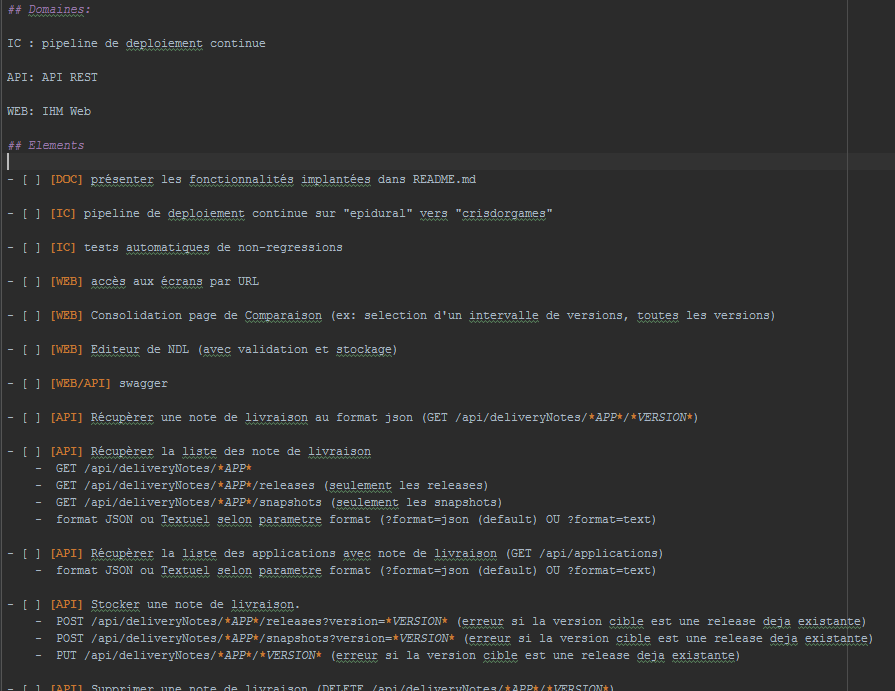
\includegraphics[width=0.6\textwidth]{backlog}
 \caption{BACKLOG}
 \label{fig:backlog}
\end{figure}

\subsection{IHM}
IHM de l'application est réalisé en Bootstrap, jQuery et GSP(le mécanismes de grails pour render views).
Il contient tous un navbar qui permet de naviger entre les pages differentes.
Le navbar contient des élements suivant:
\begin{itemize}
 \item Nom de l'application, nom de version et le numéro de déploiement sur Jenkins;
 \item Quatre buttons vers les quater pages;
 \item Un dropdown menu qui permet de swicher les languages(Français, Anglais, Chinois).
\end{itemize}

L'application contient principalement les cinq écrans suivant:

%page d'accueil
\subsubsection{La page d'accueil(fig.\ref{fig:page_home})}
Cette page contient des élements suivants:
\begin{itemize}
 \item Un bar de recherche qui ramène à la page recherche;
 \item Un modal(fig.\ref{fig:modal_setting}) pour la configuration personnalisée;
 \item Des buttons comme accès rapide vers la page recherche;
 \item Un footer qui ramène vers la documentation, les codes sources de l'applciatioini et la documentation de l'api REST.
\end{itemize}

\begin{figure}[ht]
 \centering
 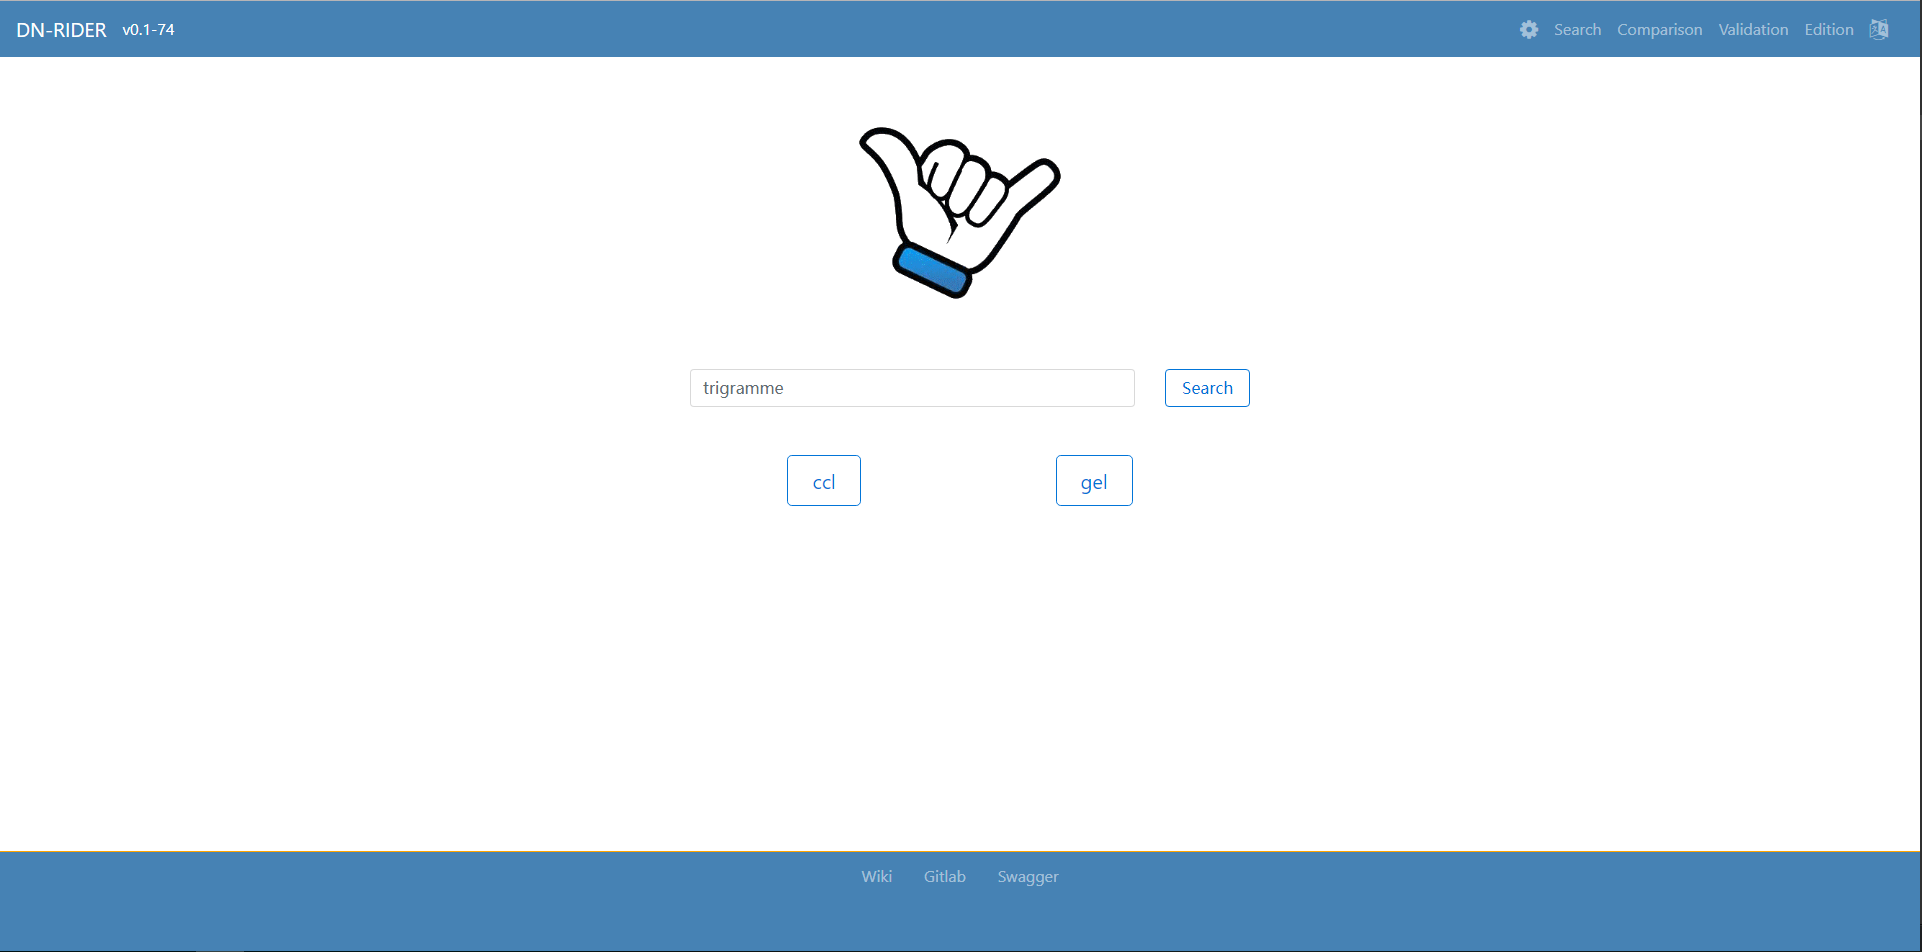
\includegraphics[width=0.8\textwidth]{page_home}
 \caption{La page d'accueil}
 \label{fig:page_home}
\end{figure}

\begin{figure}[ht]
 \centering
 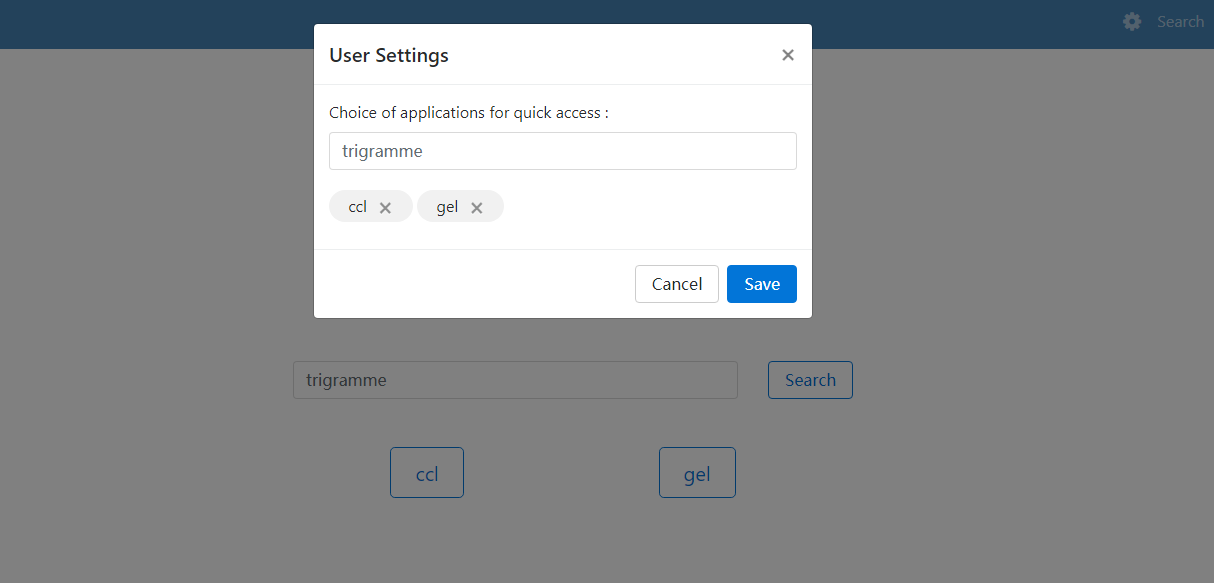
\includegraphics[width=0.6\textwidth]{modal_setting}
 \caption{Le modal configuration}
 \label{fig:modal_setting}
\end{figure}

%page recherche
\subsubsection{La page recherche(fig.\ref{fig:page_search})}
Cette page permet de choisir une notes de livraison et l'afficher.

Elle contient des élements suivants:
\begin{itemize}
 \item Un sidebar collapsible qui contient un formulaire pour choisir les notes de livraisons. On peut filter selon le type de release et la grammaire de l'expression régulier(regex);
 \item Une note de livraison affichée au format json manipulative. L'affichage de json est réalisé avec un plugin jQuery;
 \item Des buttons qui permet de swicher le format d'affichage et des liens vers la page validation et l'application Nexus.
\end{itemize}

\begin{figure}[ht]
 \centering
 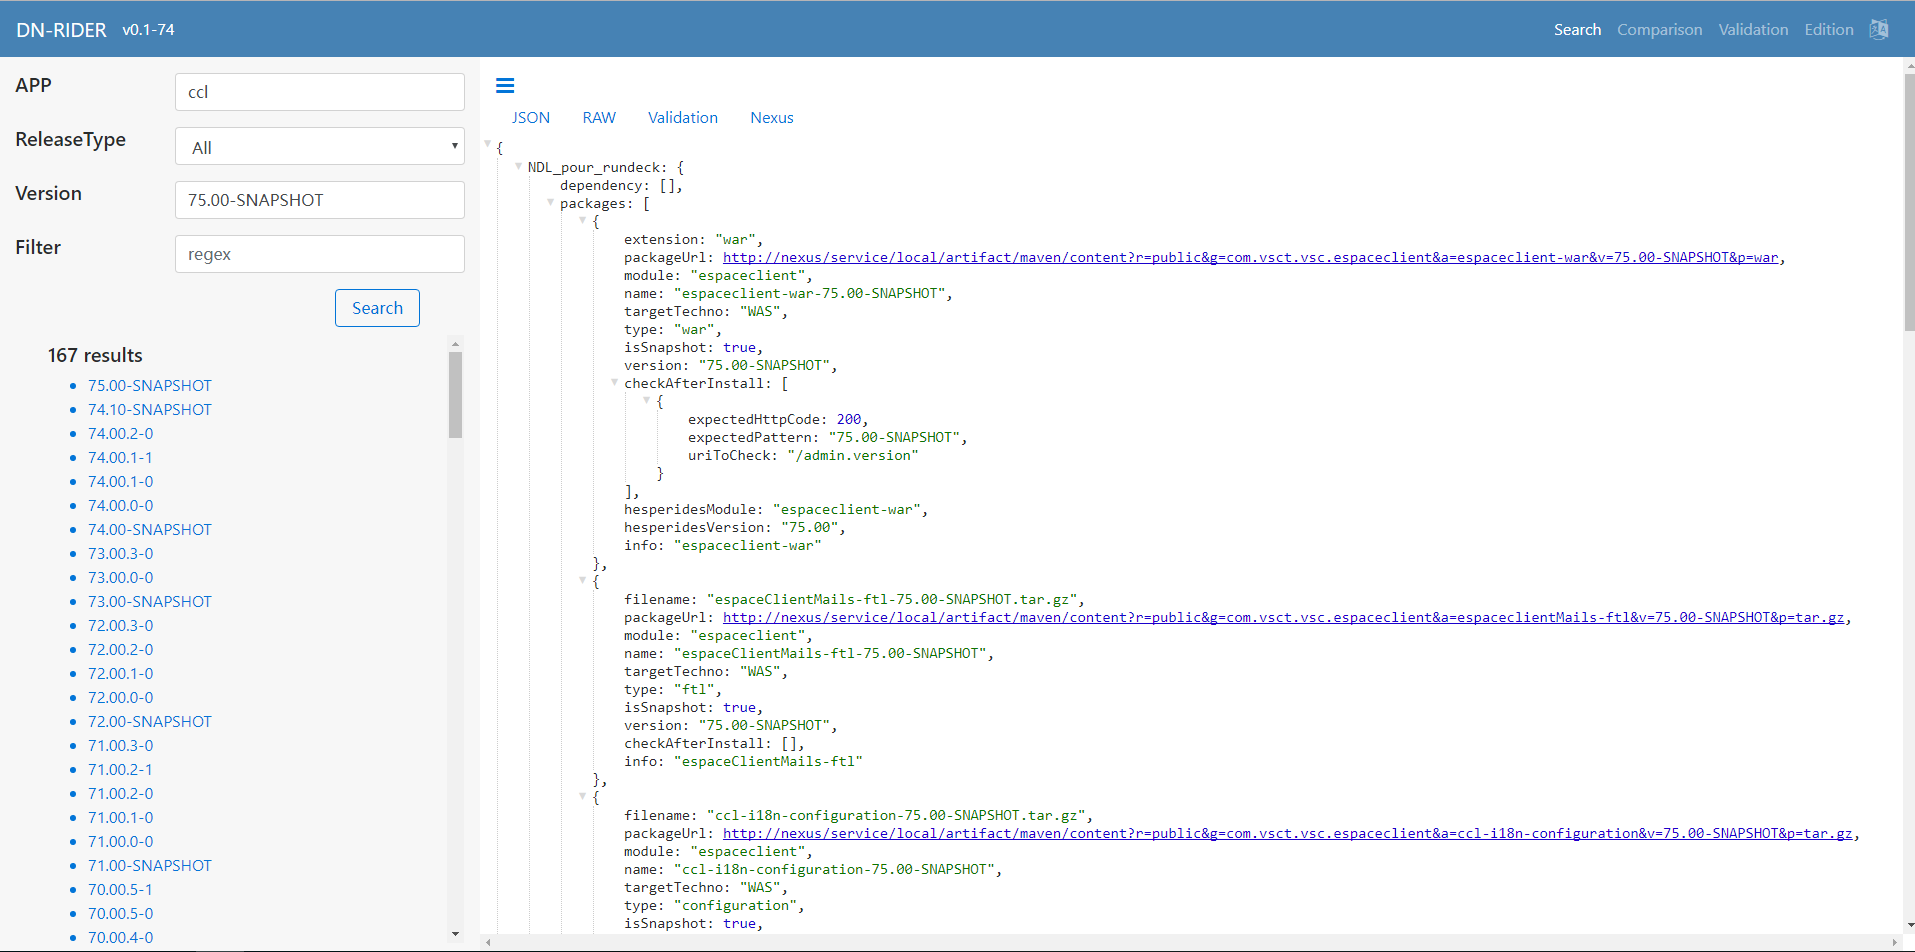
\includegraphics[width=0.8\textwidth]{page_search}
 \caption{La page recherche}
 \label{fig:page_search}
\end{figure}

%page comparaison
\subsubsection{La page comparaison(fig.\ref{fig:page_comparaison})}
Cette page permet de comparer les differents versions de notes de livraions d'une trigramme.

Elle contient des élements suivants:
\begin{itemize}
 \item Un sidebar collapsible qui contient un formulaire pour choisir les notes de livraisons;
 \item Un tableau qui compare les packages des notes de livraisons, le contenu des packages se présent dans un popover sous format json manipulatif;
\end{itemize}

\begin{figure}[ht]
 \centering
 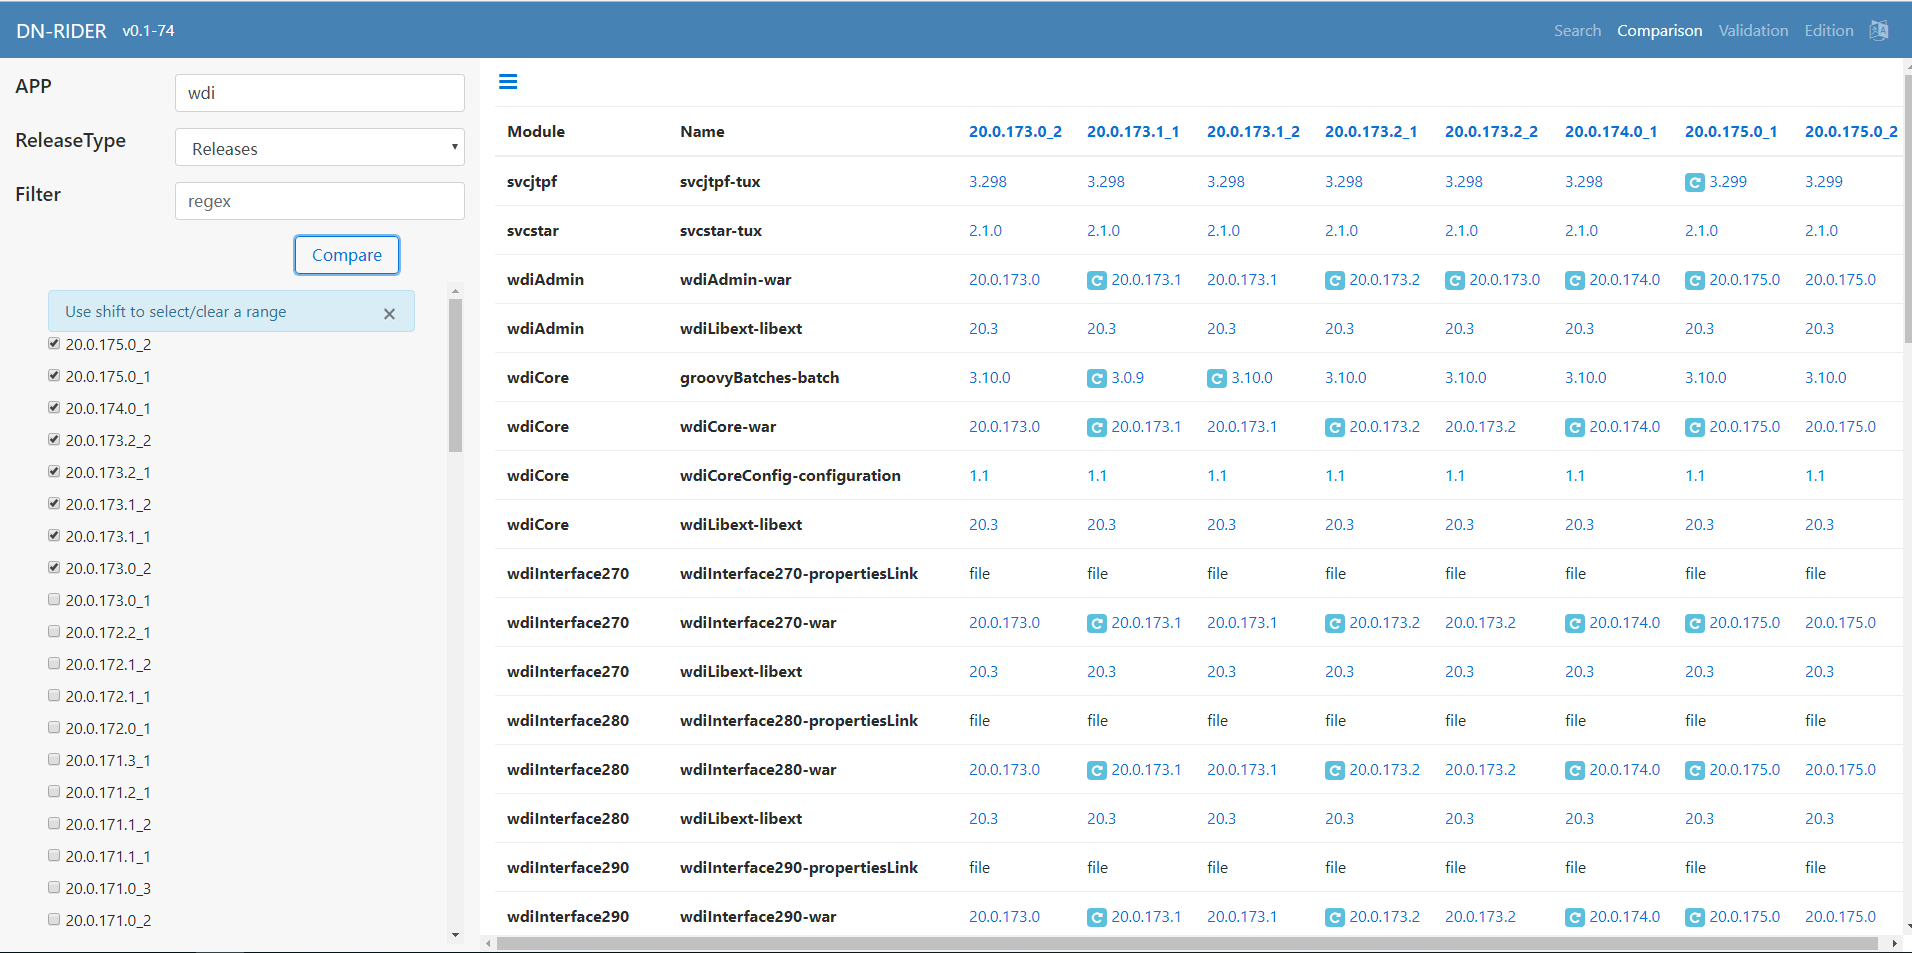
\includegraphics[width=0.8\textwidth]{page_comparison}
 \caption{La page comparaison}
 \label{fig:page_comparaison}
\end{figure}

%page validation
\subsubsection{La page validation(fig.\ref{fig:page_validation})}
Cette page permet de vérifier si une note de livraion est validée selon un json schéma.

Elle contient des élements suivants:
\begin{itemize}
 \item Une zone qui permet d'éditer une note de livraison;
 \item Un button qui ramène vers une page qui affiche le schéma;
 \item Une fênetre qui affiche les résultats de validation. Il y a trois types de résultats possibles:
       \begin{itemize}
        \item Json non valide: Afficher la postion de l'erreur et un lien vers l'erreur dans la zone d'édition;
        \item Schéma non valide: Afficher les informations erreurs détaillées au format json;
        \item Valide: Message de réussite.
       \end{itemize}
\end{itemize}

\begin{figure}[ht]
 \centering
 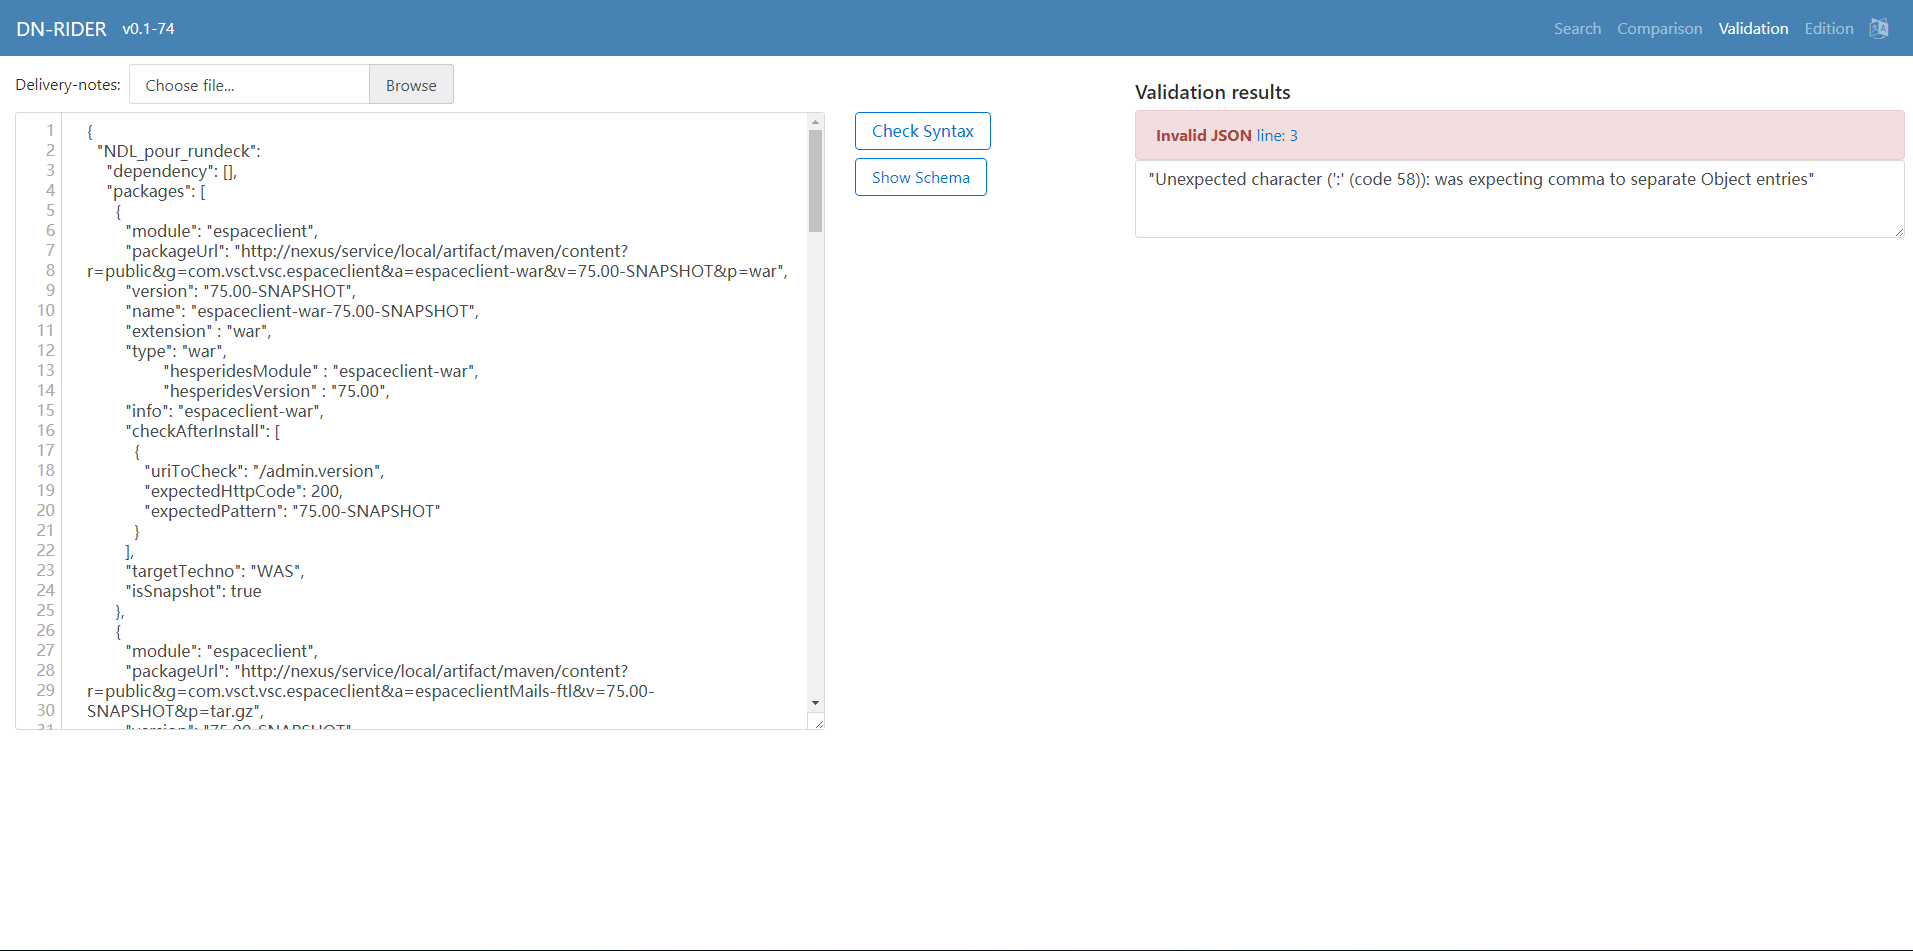
\includegraphics[width=0.8\textwidth]{page_validation}
 \caption{La page validation}
 \label{fig:page_validation}
\end{figure}

%page edition
\subsubsection{La page edition(fig.\ref{fig:page_edition})}
Cette page permet d'éditer, valider et stocker une note de livraison.

Elle contient des élements suivants:
\begin{itemize}
 \item Un sidebar collapsible qui contient un formulaire pour choisir les notes de livraisons;
 \item Une zone qui permet d'éditer une note de livraison;
 \item Une fênetre qui affiche les résultats de validation;
 \item Un modal(fig.\ref{fig:modal_save}) qui permet de stocker la note de livraison.
\end{itemize}

\begin{figure}[ht]
 \centering
 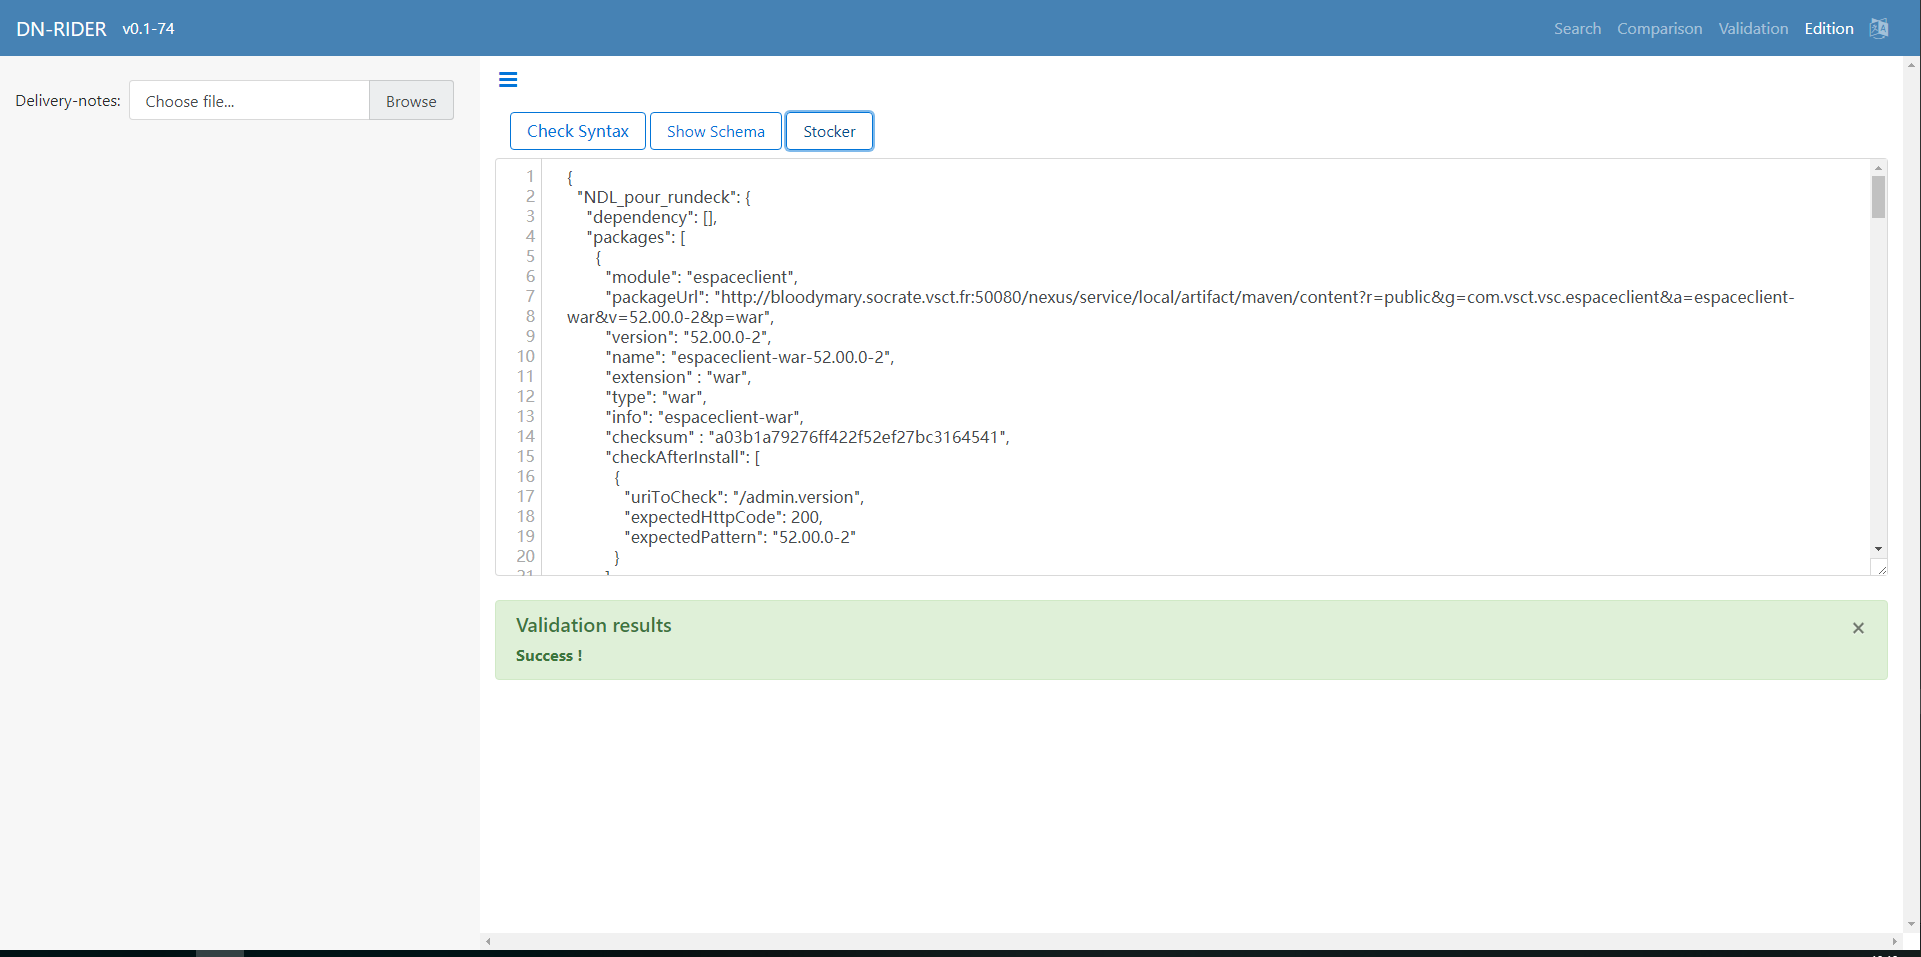
\includegraphics[width=0.8\textwidth]{page_edition}
 \caption{La page edition}
 \label{fig:page_edition}
\end{figure}

\begin{figure}[ht]
 \centering
 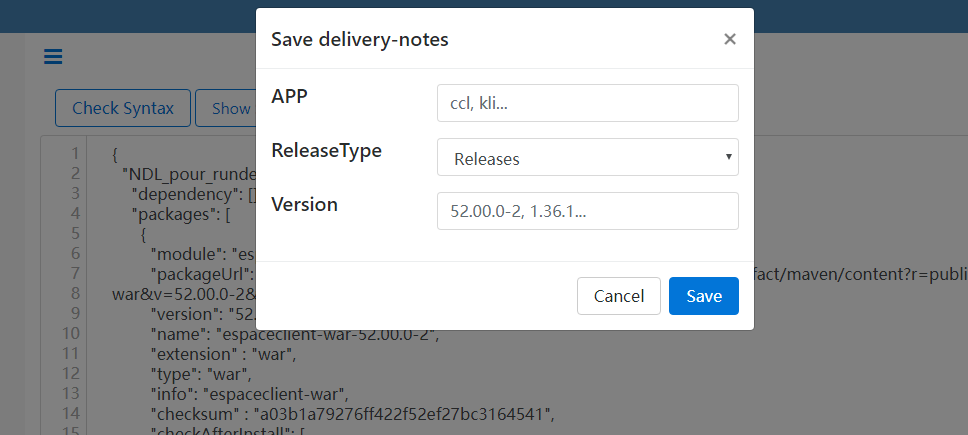
\includegraphics[width=0.6\textwidth]{modal_save}
 \caption{Le modal configuration}
 \label{fig:modal_save}
\end{figure}

\clearpage

\subsection{Api REST}
L'application fournie une interface api REST.
Comme dans l'IHM , l'api permet de chercher, valider, stocker des notes de livraison.
En plus, elle permet de supprimer des notes de livraison.
Ce qui est différent de l'IHM, on ne peut pas comparer les differents versions d'une trigramme, mais on peut obtenir le contenu d'un package d'une note de livraison.

L'application fournie aussi une interface graphique(fig.\ref{fig:page_swagger}) réalisé en Swagger pour la documentaion de l'api.
Il est réalisé en utilisant un plugin et en ajoutant des annotations dans les contrôleurs.

\begin{figure}[ht]
 \centering
 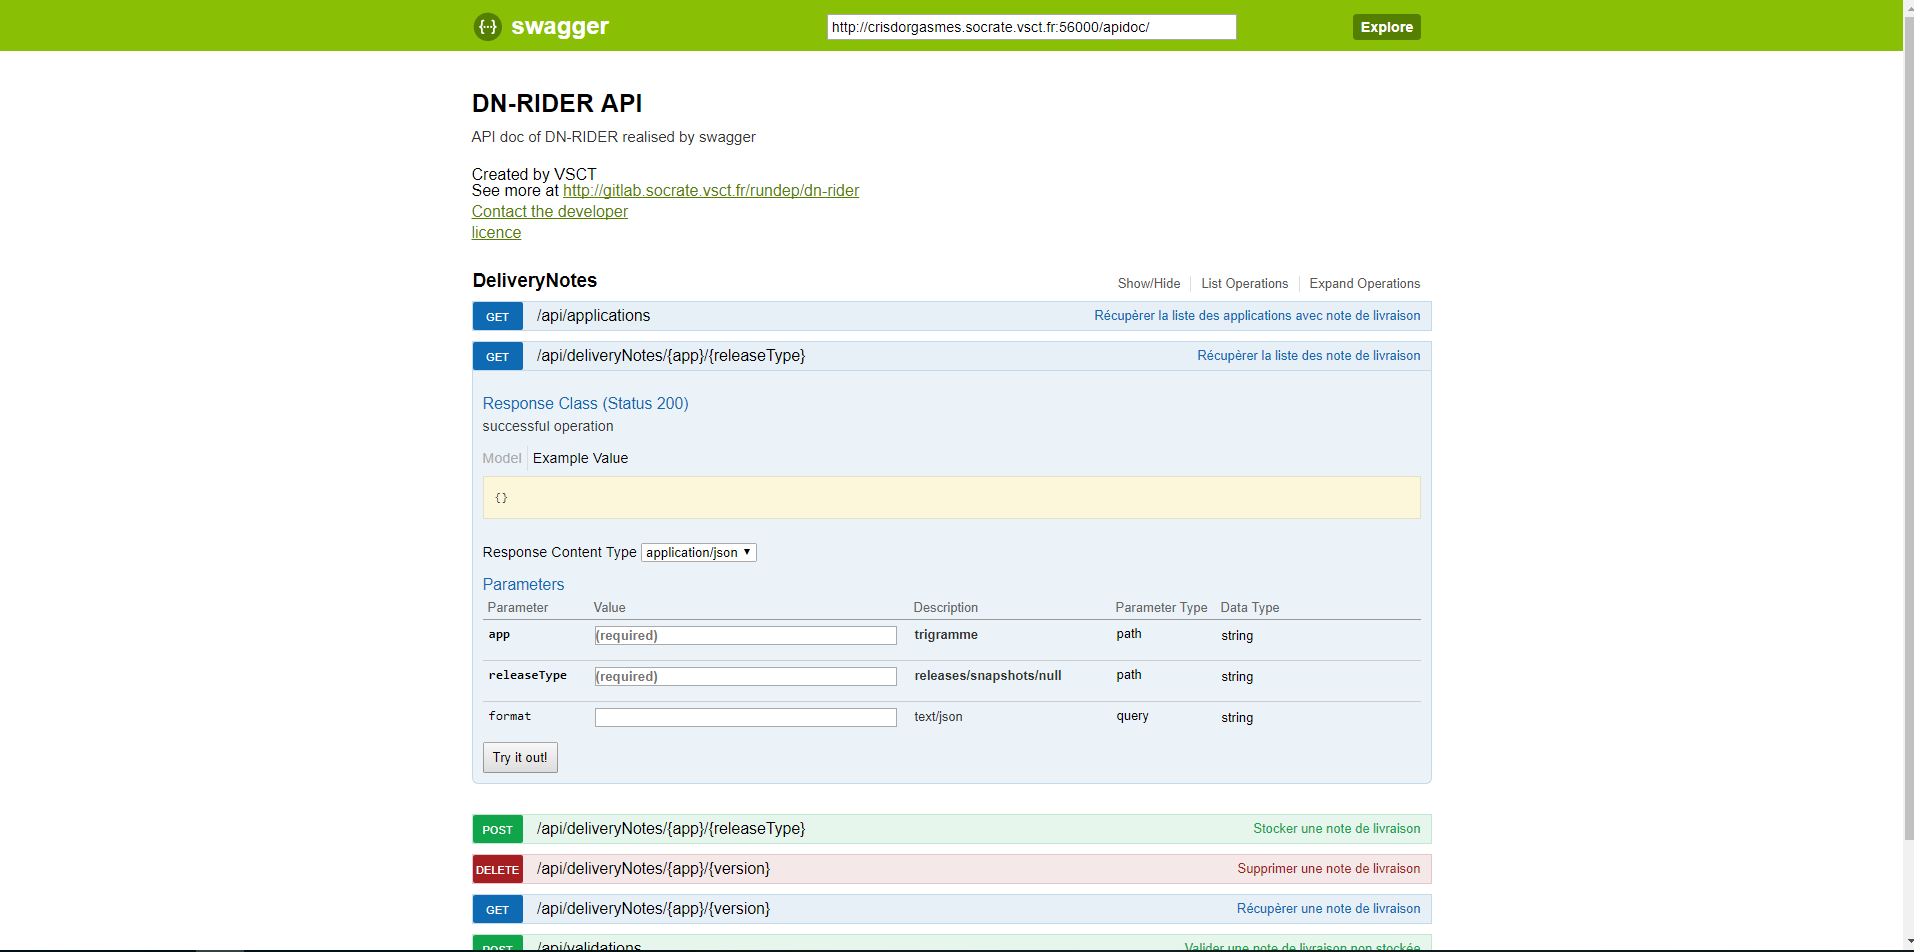
\includegraphics[width=0.8\textwidth]{page_swagger}
 \caption{La page swagger}
 \label{fig:page_swagger}
\end{figure}

\clearpage

\subsection{Intégration Continue}
Afin d'améliorer la qualité du code et du produit final et faciliter le déploiement de l'application, on pratique les principes de l'intégratioin continue.
L'intégration continus de l'application se réalise en utilisant git et jenkins pipeline.

Les codes sources sont géré en git et stocké dans Gitlab.
Au début on a défini des actions à réaliser obligatoirement avant de faire "git push":
\begin{itemize}
 \item Faire relire le code par un tiers;
 \item Faire valider par un tiers que la feature développée fonctionne comme attendu;
 \item Valider la nouvelle fonction par un ou des tests;
 \item Exécuter grails test-app.
\end{itemize}

Le pipeline(fig.\ref{fig:jenkins}) contient les étapes suivantes:
\begin{itemize}
 \item "checkout": Récupérer les codes de gitlab;
 \item "versioning": Modifier la version de l'application selon le numéro de déploiement sur Jenkins;
 \item "build": Builder l'applcation;
 \item "deploy": Copier le war excutable sur le serveur de production;
 \item "run": Excuter l'application.
\end{itemize}

\begin{figure}[ht]
 \centering
 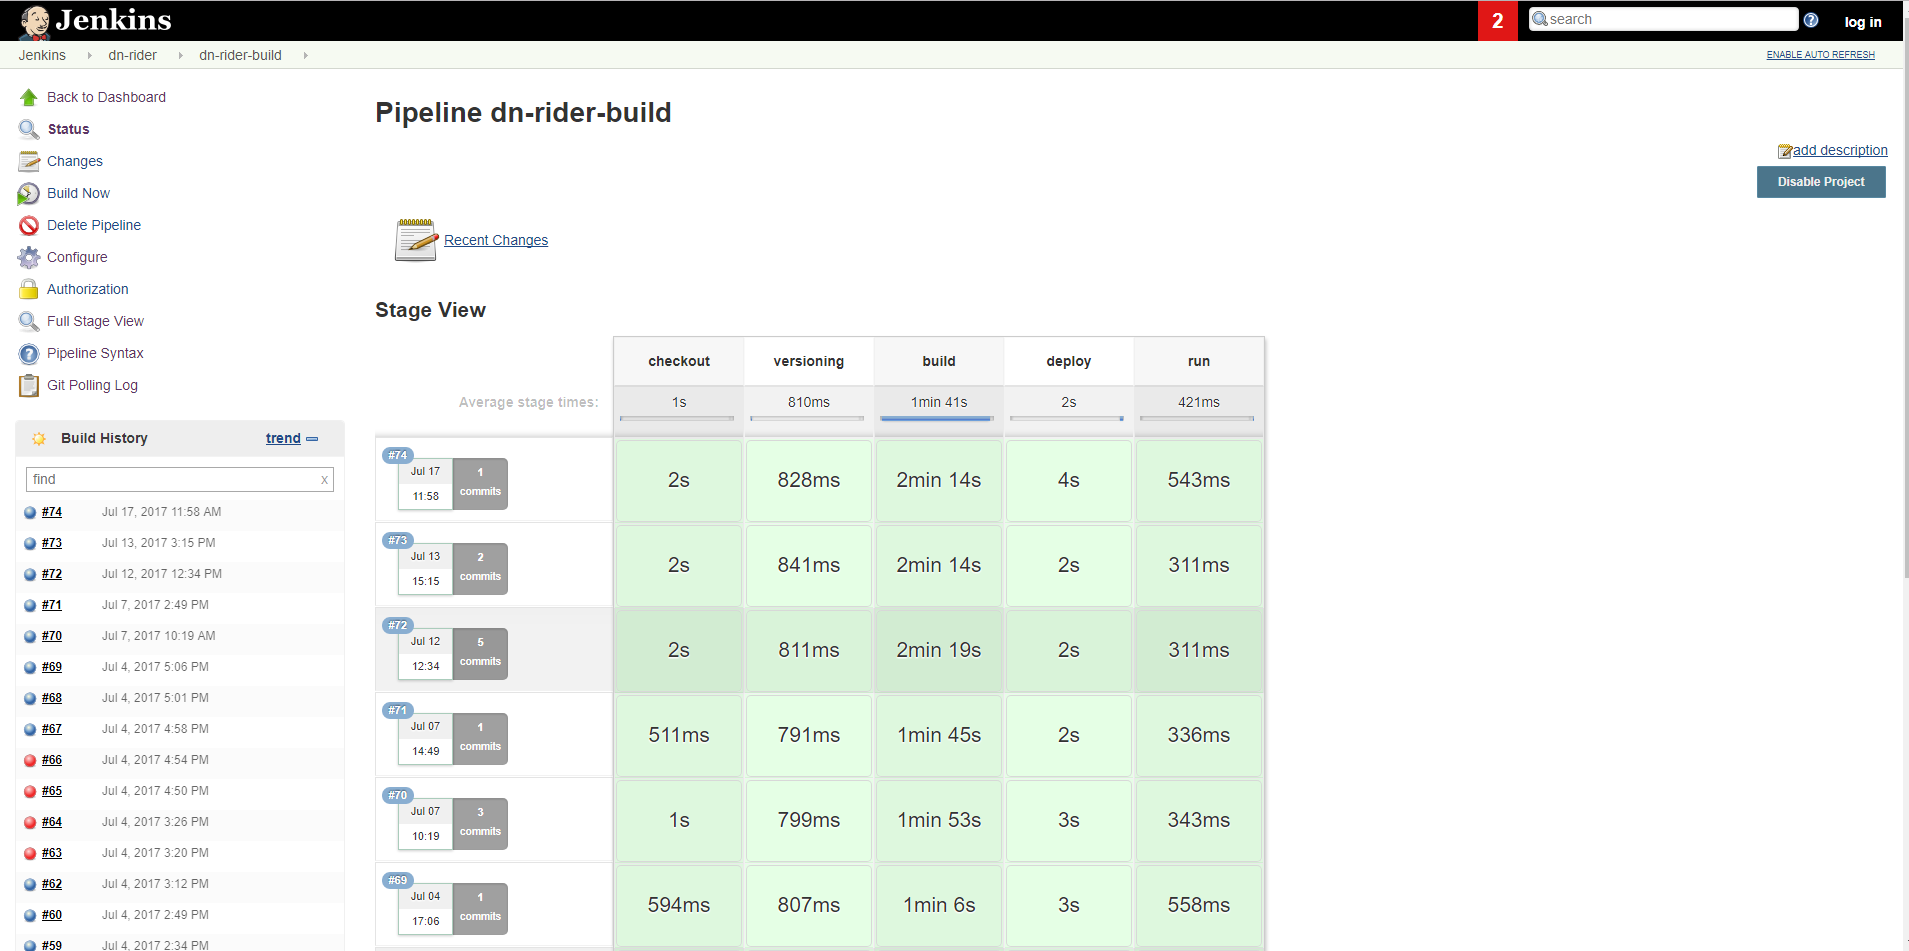
\includegraphics[width=0.8\textwidth]{jenkins}
 \caption{Jenkins}
 \label{fig:jenkins}
\end{figure}

Les tests automatique sur Jenkins sont à réaliser.

\clearpage

\clearpage
